\documentclass{article}
\usepackage[english]{babel}
\usepackage{geometry,amsmath,amssymb,graphicx,alltt}
\geometry{a4paper}

%%%%%%%%%% Start TeXmacs macros
\newcommand{\tmaffiliation}[1]{\\ #1}
\newcommand{\tmop}[1]{\ensuremath{\operatorname{#1}}}
\newcommand{\tmtextit}[1]{\text{{\itshape{#1}}}}
\newenvironment{tmcode}[1][]{\begin{alltt} }{\end{alltt}}
%%%%%%%%%% End TeXmacs macros

\begin{document}

\title{Machine learning}

\author{
  Youjun Hu
  \tmaffiliation{yjhu@ipp.cas.cn}
}

\maketitle

\

\section{Introduction}

Artificial intelligence (AI) research has tried many different approaches
since its founding. In the first decades of the 21st century, the AI research
is dominated by highly mathematical optimization machine learning (ML), which
has proved successful in solving many challenging real life problems.

Many problems in AI can be solved theoretically by searching through many
possible solutions: Reasoning can be reduced to performing a search. Simple
exhaustive searches are rarely sufficient for most real-world problems. The
solution, for many problems, is to use "heuristics" or "rules of thumb" that
prioritize choices in favor of those more likely to reach a goal. A very
different kind of search came to prominence in the 1990s, based on the
mathematical theory of optimization. Modern machine learning is based on these
methods. Instead, of using detailed explanations to guide the search, it uses
a combination of{\cite{nielsen2015neural}}: (a) general architectures; (b)
trying trillions of possibilities, guided by simple ideas (like gradient
descent) for improvement; and (c) the ability to recognize progress (by
defining a objective function).

I am interested in applying machine learning to problems in computational
physics problems that traditional numerical methods can not easily handle
either because of its computational costs being too high or its traditional
algorithms are too complicated to easily implement.

Enrico Fermi once criticized the complexity of a model (that contains many
free parameters) by quoting Johnny von Neumann ``With four parameters I can
fit an elephant, and with five I can make him wiggle his trunk''. What Fermi
implies is that it is easy to fit existing data and what is important is to
have a model with predicting capability (fitting data not seen yet). The
artificial neural network method tackles this difficulty by increasing the
number of free parameters to millions, with the hope of obtaining predicting
capability.

\section{Neural network}

Neural networks consists of multiple layers of interconnected nodes (neurons),
each having a weight for a connection, a bias, and an activation function.
Each layer build upon the previous layer. This progression of computations
through the network is called forward propagation. Another process called
backpropagation uses algorithms which moves backwards through the layers to
efficiently compute the partial derivatives of the objective function with
respect to the weights and biases. Combining the forward and backward
propagation, we can calculate errors in predictions and then adjusts the
weights and biases using the gradient descent method. This process is called
training/learning.

\subsection{ Node (neuron or unit), weight, bias, and activation}

As is shown in Fig. \ref{22-3-13-a1}, we use $w_{j k}^l$ to denote the weight
for the connection from the $k^{\tmop{th}}$ neuron in the $(l -
1)^{\tmop{th}}$ layer to the $j^{\tmop{th}}$ neuron in the $l^{\tmop{th}}$
layer. Use $b_j^l$ to denote the bias of the $j^{\tmop{th}}$ neuron in the
$l^{\tmop{th}}$ layer.

\begin{figure}[h]
  \raisebox{-0.369502148506993\height}{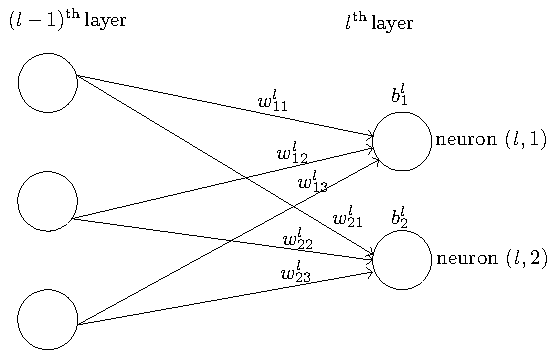
\includegraphics[width=9.35164961301325cm,height=5.99124360487997cm]{machine_learning-1.pdf}}
  \caption{\label{22-3-13-a1}Definition of layers, neurons, weights, and
  biases in a neural network. The $j^{\tmop{th}}$ neuron in the
  $l^{\tmop{th}}$ layer is referred to as neuron $(l, j)$}
\end{figure}

\

We use $a_j^l$ to denote the output (activation) of the $j^{\tmop{th}}$
neuron in $l^{\tmop{th}}$ layer. A neural network model assumes that $a_j^l$
is related to the $a^{l - 1}$ (output of the previous layer) via
\begin{equation}
  \label{22-3-9-e2} a^l_j = \sigma \left( \sum_k w_{j k}^l a^{l - 1}_k + b^l_j
  \right),
\end{equation}
where the summation is over all neurons in the $(l - 1)^{\tmop{th}}$ layer and
$\sigma$ is a function called activation function which can take various
forms, e.g., step function,
\begin{equation}
  \sigma (z) = \left\{ \begin{array}{l}
    1 \tmop{if} z \geqslant 0\\
    0 \quad \tmop{else}
  \end{array} \right.,
\end{equation}
rectified linear unit (ReLU),
\begin{equation}
  \sigma (z) = \max (0, z),
\end{equation}
and sigmoid (``S''-shaped curve, also called logistic function)
\begin{equation}
  \label{23-7-28-p1} \sigma (z) = \frac{1}{1 + \exp (- z)} .
\end{equation}
For natation ease, define $z_j^l$ by
\begin{equation}
  \label{22-3-9-1} z^l_j = \sum_k w_{j k}^l a^{l - 1}_k + b^l_j,
\end{equation}
which can be interpreted as an weighted input to the neuron $(l, j)$, then Eq.
(\ref{22-3-9-e2}) is written as
\begin{equation}
  a_j^l = \sigma (z^l_j) .
\end{equation}
In matrix form, Eq. (\ref{22-3-9-1}) is written as
\begin{equation}
  z^l = w^l a^{l - 1} + b^l,
\end{equation}
where $w^l$ is a $J \times K$ matrix, $z^l$ \ and $b^l$ are column vectors of
length $J$, $a^{l - 1}$ is a column vector of length $K$, where $J$ and $K$
are the number of neurons in the $l^{\tmop{th}}$ layer and $(l -
1)^{\tmop{th}}$ layer, respectively.

The input layer is where data inputs are provided, and the output layer is
where the final prediction is made. The input and output layers of a deep
neural network are called visible layers. The layers between the input layer
and output layer are called hidden layers. Note that the input layer is
usually not considered as a layer of the network since it does not involve any
computation. In tensorflow, layers refer to the computing layers (i.e., hidden
layers and the output layer, not including the input layer). The activation
function of each layer can be different. The activation function of the output
layer is often chosen as None, ReLU, logistic/tanh, and is usually different
from those used in the hidden layers. Here ``None'' means activation $\sigma
(z) = z$.

\subsection{Objective function}

Define an objective function (can be called loss or cost function depending on
contexts) by
\begin{equation}
  \label{22-3-9-e1} C (w, b) \equiv \frac{1}{2 n} \sum_x \| y (x) - a^L \|^2,
\end{equation}
where $w$ and $b$ denotes the collection of all weights and biases in the
network, $n$ is the total number of training examples $x$, the summation is
over all the training examples, $y (x)$ is the desired output from the network
(i.e., correct answer) when $x$ is the input, and $a^L$ is the actual output
from the output layer of the network and is a function of $w, b$, and $x$.
Note that $y$ and $a^L$ are vectors (with number of elements being the number
of neurons in the output layer) and $\| \ldots \|$ denotes the vector norm.
Explicitly writing out the vector norm, Eq. (\ref{22-3-9-e1}) is written as
\begin{equation}
  \label{22-3-9-e1m} C (w, b) \equiv \frac{1}{2 n} \sum_x \sum^{N_L}_{j = 1}
  (y_j (x) - a^L_j)^2,
\end{equation}
where $N_L$ is the number of neurons in the output layer.

The cost function is the average error of the approximate solution away from
the desired exact solution. The goal of a learning algorithm is to find
weights and biases that minimize the cost function. A method of minimizing the
cost function over $(w, b)$ is the gradient descent method:
\begin{equation}
  w_{j k}^l \rightarrow w_{j k}^l - \eta \frac{\partial C}{\partial w_{j
  k}^l},
\end{equation}

\begin{equation}
  b_j^l \rightarrow b_j^l - \eta \frac{\partial C}{\partial b_j^l},
\end{equation}
where $\eta$ is called learning rate, which should be positive.

In using the gradient descent method, we need to compute the partial
derivatives $\partial C / \partial w^l_{j k}$ and $\partial C / \partial
b^l_j$. Next we will discuss how to compute them.

\subsection{Gradients of objective function}

Note that the loss function involves an average over all the training
examples. Denote the loss function for a specific training example by $C_x$,
i.e.,
\begin{equation}
  \label{22-3-11-a6} C_x = \frac{1}{2} \sum^{N_L}_{j = 1} (y_j (x) - a^L_j)^2,
\end{equation}
then expression (\ref{22-3-9-e1m}) is written as
\begin{equation}
  C = \frac{1}{n} \sum_x C_x,
\end{equation}
Then the partial derivatives $\partial C / \partial w^l_{j k}$ and $\partial C
/ \partial b^l_j$ can be written as the sum of $\partial C_x / \partial w^l_{j
k}$ and $\partial C_x / \partial b^l_j$, i.e.,
\begin{equation}
  \label{22-3-11-a3} \frac{\partial C}{\partial w_{j k}^l} = \frac{1}{n}
  \sum_x \frac{\partial C_x}{\partial w_{j k}^l},
\end{equation}

\begin{equation}
  \label{22-3-11-a4} \frac{\partial C}{\partial b_j^l} = \frac{1}{n} \sum_x
  \frac{\partial C_x}{\partial b_j^l} .
\end{equation}
The above formulas indicate that, once $\partial C_x / \partial w^l_{j k}$ and
$\partial C_x / \partial b^l_j$ are known, obtaining \ $\partial C / \partial
w^l_{j k}$ and $\partial C / \partial b^l_j$ is trivial, i.e., just averaging
them. Therefore, we will focus on $C_x$ (i.e., the cost function for a fixed
training example) and discuss how to compute $\partial C_x / \partial w^l_{j
k}$ and $\partial C_x / \partial b^l_j$.

In practice, we do not sum over all the training examples. Instead, we
average the derivative over a small number (say 16) of training examples (a
mini batch) and use these approximate derivatives to advance a step. For the
next step, we stochastically change to using a different mini batch. This is
called stochastic gradient descent (SGD) method.

\subsection{Back-propagating algorithm}

The cost function $C_x$ is a function of weights and biases of all neurons
(the input $x$ and output $y (x)$ are fixed parameters). For a specific neuron
$(l, j)$, its weights and biases enter $C_x$ via the combination $z_j^l =
\sum_k w_{j k}^l a^{l - 1}_k + b^l_j$. Then it is useful to define the
following partial derivative:
\begin{equation}
  \label{22-3-11-p1} \delta^l_j \equiv \frac{\partial C_x}{\partial z_j^l},
\end{equation}
where the partial derivative are taken with fixed weights and biases for all
neurons except neuron $(l, j)$. Note that the $a_k^{l - 1}$ appearing in the
expression of $z_j^l$ does not depend on $w^l_{j k}$ or $b^l_j$. It only
depends on the weights and biases in the layers $\leqslant (l - 1)$, which are
all fixed when taking the derivative in expression (\ref{22-3-11-p1}).
$\delta^l_j$ defined in expression (\ref{22-3-11-p1}) is often called the
error of neuron $(l, j)$.

Using the chain rule, \ $\partial C_x / \partial w^l_{j k}$ and $\partial C_x
/ \partial b^l_j$ can be expressed in terms of $\delta^l_j$:
\begin{equation}
  \frac{\partial C_x}{\partial b_j^l} = \frac{\partial C_x}{\partial z_j^l} 
  \frac{\partial z^l_j}{\partial b_j^l} = \delta^l_j,
\end{equation}
and
\begin{equation}
  \frac{\partial C_x}{\partial w_{j k}^l} = \frac{\partial C_x}{\partial
  z_j^l}  \frac{\partial z^l_j}{\partial w_{j k}^l} = \delta^l_j a_k^{l - 1} .
\end{equation}
Therefore, if $\delta^l_j$ is known, it is trivial to compute the gradients
needed in the gradient descent method.



\

\raisebox{-0.369502148506993\height}{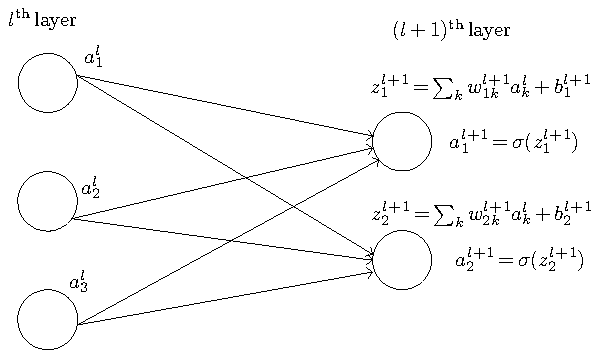
\includegraphics[width=10.0733799029254cm,height=5.99124360487997cm]{machine_learning-2.pdf}}

\

\

\

For the output layer ($L^{\tmop{th}}$ layer), $\delta^l_j$ defined in Eq.
(\ref{22-3-11-p1}) is written as
\begin{equation}
  \delta^L_j = \frac{\partial C_x}{\partial z_j^L} = \frac{\partial
  C_x}{\partial a^L_j}  \frac{\partial a^L_j}{\partial z_j^L} .
\end{equation}
The dependence of $C_x$ on $a_j^L$ is explicitly given by Eq.
(\ref{22-3-11-a6}), from which the above expression for $\delta_j^L$ is
written as
\begin{equation}
  \delta^L_j = (a^L_j - y_j (x)) \sigma' (z_j^L) .
\end{equation}
Therefore $\delta^L_j$ is easy to compute.

Backpropagation is a way of computing $\delta^l_j$ for every layer using
recurrence relations: the relation between $\delta^l$ and $\delta^{l + 1}$.
Noting how the error is propagating through the network, we know the following
identity:
\begin{equation}
  \frac{\partial C_x}{\partial z_J^l} d z^l_J = \sum_j \frac{\partial
  C_x}{\partial z_j^{l + 1}} d z^{l + 1}_j,
\end{equation}
with
\begin{equation}
  d z_j^{l + 1} = w^{l + 1}_{j J} d (a^l_J),
\end{equation}
i.e.,
\begin{equation}
  d z_j^{l + 1} = w^{l + 1}_{j J} \sigma' (z^l_J) d z^l_J .
\end{equation}
Therefore
\begin{equation}
  \frac{\partial C_x}{\partial z_J^l} = \sum_j \frac{\partial C_x}{\partial
  z_j^{l + 1}} w^{l + 1}_{j J} \sigma' (z^l_J) .
\end{equation}
i.e.,
\begin{equation}
  \label{22-3-14-a1} \delta^l_J = \sum_j \delta^{l + 1}_j w^{l + 1}_{j J}
  \sigma' (z^l_J) .
\end{equation}
Equation (\ref{22-3-14-a1}) gives the recurrence relations of computing
$\delta^l$ from $\delta^{l + 1}$. This is called the backpropagation
algorithm. Eq. (\ref{22-3-14-a1}) can be written in the matrix form:
\begin{equation}
  \delta^l = ((w^{l + 1})^T \delta^{l + 1}) \odot \sigma' (z^l),
\end{equation}
where $T$ stands for matrix transpose, $\odot$ is the element-wise product.

\

\section{Automatic differentiation}

Automatic differentiation (autodiff) is a set of techniques for computing
derivatives of numeric functions expressed as source code (i.e. the internal
mechanism of the function is known). It works by breaking down functions into
elementary operations (addition, multiplication, etc.) whose derivatives are
known, and then applies the chain rule to compute the derivatives.

Autodiff can be considered as a kind of symbolic differentiation. The
difference of autodiff from the traditional symbolic differentiaton is that
the goal is not to get a compact formula for humans to understand, but for
computers to evaluate. Therefore the final result from a autodiff is not an
analytical formula, but numerical data. This goal also makes autodiff more
efficient since autodiff doses not need to perform some intermedia processes
that appear when you use traditional symbolic differentiation to get a formula
and then numerically evaluate the formula.

Autodiff can be better than numerical differentiation (e.g., finite
difference) in that it avoid truncation errors. When you are given a black-box
function, you can not use autodiff since the internal mechinism of the
function is unknown. In this case, the only choice is to use numerical
differentiation.

Autodiff has two main modes: forward and backward. Forward mode computes a
single derivative during one pass of the expression tree. The back mode
computes all the derivatives in a single pass of the expression tree, avoiding
some computational repetition (compared using forward mode to compute all the
derivatives sperately). It's more efficient for functions with many inputs and
few outputs, making it ideal for machine learning where we often compute
gradients of scalar loss functions with respect to many parameters.
Backpropagation is a specific instance of backward-mode autodiff. Here is a
simple Python code implementing autodiff:

\

Forward:
\begin{tmcode}
class Expression:
    def __add__(exp1, exp2):
        return Plus(exp1, exp2)
    def __mul__(exp1, exp2):
        return Multiply(exp1,exp2)
class Variable(Expression):
    def __init__(self,value):
        self.value = value
    def evaluate(self):
        return self.value
    def derive(self, v):
        return 1 if self == v else 0

class Plus(Expression):
    def __init__(self,exp1,exp2):
        self.a = exp1
        self.b = exp2
    def evaluate(self):
        return self.a.evaluate() + self.b.evaluate()
    def derive(self,v):
        return self.a.derive(v) + self.b.derive(v)

class Multiply(Expression):
    def __init__(self,exp1,exp2):
        self.a = exp1
        self.b = exp2
    def evaluate(self):
        return self.a.evaluate() * self.b.evaluate()
    def derive(self, v):
        return (self.a.derive(v)*self.b.evaluate() 
               +self.b.derive(v)*self.a.evaluate())

# Example: derivatives of z(x,y) at (x, y) = (2, 3)
x = Variable(2)
y = Variable(3)
z = x * (x + y) + y * y
print(z.derive(x)) # dz/dx,  Output: 7
print(z.derive(y)) # dz/dy,  Output: 8
\end{tmcode}
This simple example illustrates several important concepts:

* Class, subclass, inheritance

* Operator overloading

* Polymorphism

* Recursion

\

The following is the backward (or reverse) method.
\begin{tmcode}
class Expression:
    def __add__(exp1, exp2):
        return Plus(exp1,exp2)
    def __mul__(exp1, exp2):
        return Multiply(exp1, exp2)
        
class Variable(Expression):
    def __init__(self,value):
        self.value = value
        self.partial = 0
    def evaluate(self):
        return self.value
    def derive(self,seed):
        self.partial += seed

class Plus(Expression):
    def __init__(self,exp1,exp2):
        self.a = exp1
        self.b = exp2
    def evaluate(self):
        return self.a.evaluate() + self.b.evaluate()
    def derive(self,seed):
        self.a.derive(seed)
        self.b.derive(seed)
        
class Multiply(Expression):
    def __init__(self,exp1,exp2):
        self.a = exp1
        self.b = exp2
    def evaluate(self):
        return self.a.evaluate() * self.b.evaluate()
    def derive(self,seed):
        self.a.derive(seed * self.b.evaluate())
        self.b.derive(seed * self.a.evaluate())

x = Variable(2)
y = Variable(3)
z = x * (x + y) + y * y
z.derive(1)
print(x.partial)  # dz/dx Output:  7
print(y.partial)  # dz/dy Output:  8
\end{tmcode}
Another method is to use dual numbers. Dual number are expressions of the form
$a + b \varepsilon$, where $a$ and $b$ are real numbers, and $\varepsilon$ is
a symbol taken to satisfy $\varepsilon^2 = 0$ with $\varepsilon \neq 0$. Using
a dual number in the Taylor series, we obtain
\begin{equation}
  f (a + b \varepsilon) = \sum_{n = 0}^{\infty} \frac{f^{(n)} (a)}{n!} (b
  \varepsilon)^n = f (a) + b f' (a) \varepsilon,
\end{equation}
since all terms invovling $\varepsilon^2$ and greater powers are zero by the
defintion of $\varepsilon$. We find the coefficient of $\varepsilon$ in the
result is the first derivative $f' (a)$. This result can be used in computer
programs to find derivative of a function by defining a class and overloading
the basic operators, e.g.
\begin{equation}
  a_1 + b_1 \varepsilon + a_2 + b_2 \varepsilon = (a_1 + a_2) + (b_1 + b_2)
  \varepsilon,
\end{equation}
\begin{equation}
  (a_1 + b_1 \varepsilon) \star (a_2 + b_2 \varepsilon) = a_1 a_2 + (a_1 b_2 +
  a_2 b_1) \varepsilon .
\end{equation}
Here is a Python code:
\begin{tmcode}
class Dual:
    def __init__(self, realPart, infs=0):
        self.realPart = realPart
        self.infs = infs

    def __add__(self, other):
        return Dual(
            self.realPart + other.realPart,
            self.infs + other.infs
        )

    def __mul__(self, other):
        return Dual(
            self.realPart * other.realPart,
            other.realPart * self.infs + self.realPart * other.infs
        )

def f(x, y):
    return x * (x + y) + y * y
x = Dual(2)
y = Dual(3)
epsilon = Dual(0, 1)
a = f(x + epsilon, y)
b = f(x, y + epsilon)
print("dz/dx =", a.infs)  # Output: dz/dx= 7
print("dz/dy =", b.infs)  # Output: dz/dy = 8
\end{tmcode}


\section{misc}

\section{Least square}

In the least square method, the loss function is defined as
\begin{equation}
  L = \sum_{i = 1}^n | \hat{\mathbf{y}} (\mathbf{x}_i) -\mathbf{y}_i |^2,
\end{equation}
where $\hat{\mathbf{y}} (\mathbf{x}_i)$ is the output of the model for the
input $\mathbf{x}_i$, $n$ is the number of data points.

In the most general case, each data point considers of multiple independent
variables and multiple dependent variables $(\mathbf{x}, \mathbf{y})$. In
simple cases, each data point has one independent variable and one dependent
variable. For example, a data set consists of \tmtextit{n} data-points $(x_i,
y_i)$, \tmtextit{i} = 1, {\ldots}, \tmtextit{n}, where $x_i$ is an independent
variable and $y_i$ is a dependent variable whose value is found by
observation. The model function has the form $y (x) = f (x, \mathbf{\beta})$,
where \tmtextit{m} adjustable parameters are held in the vector
$\mathbf{\beta}$. A least squar model is called linear if the model comprises
a linear combination of the parameters, i.e.,
\begin{equation}
  f (x, \mathbf{\beta}) = \sum_{j = 1}^m \beta_j \varphi_j (x),
\end{equation}
where $\varphi_j (x)$ are basis functions chosen. Letting $X_{i j} = \varphi_j
(x_i)$, then the model prediction for input $x_i$ can be written as
\begin{equation}
  f_i \equiv f (x_i, \mathbf{\beta}) = \sum_{j = 1}^m X_{i j} \beta_j .
\end{equation}
For $n$ data points, the above can be written in matrix form:
\begin{equation}
  \mathbf{f}=\mathbf{X}\mathbf{\beta},
\end{equation}
where $\mathbf{f}= (f_1, \ldots f_n)^T$.

For linear least-square fitting, we can solve the ``normal equation'' to get
the fitting coefficients. Alternatively, one can use iterative methods, e.g.,
the gradient descent method, to minimize the mean square error over the
coefficients. The following is a complete example in Python:
\begin{tmcode}
import numpy as np
import matplotlib.pyplot as plt
class Linear_Regression:
    def __init__(self):
            self.b = [0, 0]
            
    def predict(self, X):
            Y_pred = self.b[0] + self.b[1]*X
            return Y_pred

    def update_coeffs(self, X, Y, learning_rate):
            Y_pred = self.predict(X)
            m = len(Y)
            self.b[0] = self.b[0] - (learning_rate * ((1/m) *
                                                      np.sum(Y_pred - Y)))
            self.b[1] = self.b[1] - (learning_rate * ((1/m) *
                                                      np.sum((Y_pred - Y) * X)))
 
 
regressor = Linear_Regression()
Nd=11
X = np.array([i for i in range(Nd)])
Y = np.array([2*i for i in range(Nd)]) + np.random.uniform(high=5.0,size=Nd)
fig, ax = plt.subplots()
ax.plot(X,Y, 'k.',label='data') 
Y_pred = regressor.predict(X)
ax.plot(X, Y_pred, label='Initial fit line')

learning_rate = 0.01
i = 0
while i<100:
    regressor.update_coeffs(X,Y,learning_rate)
    i = i+1

Y_pred = regressor.predict(X)
ax.plot(X, Y_pred, 'b-',label='Final Fit Line')
ax.legend()
plt.show()
\end{tmcode}
The loss function is defined by the mean square error, which \ is not directly
used in the above code. Only the partial derivatives of the loss function is
directly used.

\section{Logistic regression for binary classification}

Hypothesis function (the model): Denote the output of the model by $\hat{y}$,
which is given by
\begin{equation}
  \hat{y} = \sigma (z),
\end{equation}
where $z = w \cdot x + b$ and $\sigma$ is the sigmoid function given by Eq.
(\ref{23-7-28-p1}). The model is nonlinear in the unknowns $w$ and $b$.

The loss function is chosen as
\begin{equation}
  L = - \frac{1}{m} \sum_{i = 1}^m [y_i \log (\hat{y}_i) + (1 - y_i) \log (1 -
  \hat{y}_i)],
\end{equation}
where $y_i$ is the correct answer of the $\tmop{ith}$ training example ($y_i$
can take only two values, 0 or 1). The value of $\widehat{y_i}$ is interpreted
as the probability of $y$ being 1.

Because the model function is nonlinear and the loss function is complicated,
there is usually no closed-form solution that minimizes the loss function.
Iterative methods, such as gradient descent, are needed to solve for $w$ and
$b$. The partial derivatives needed in the gradient desent method can be
written as
\begin{eqnarray}
  \frac{\partial L}{\partial w} & = & - \frac{1}{m} \sum_i \left[ y_i 
  \frac{1}{\hat{y}_i} \sigma' (z) x_i - (1 - y_i) \frac{1}{(1 - \hat{y}_i)}
  \sigma' (z) x_i \right] \nonumber\\
  & = & - \frac{1}{m} \sum_i \left\{ \left[ y_i  \frac{1}{\hat{y}_i} - (1 -
  y_i) \frac{1}{(1 - \hat{y}_i)} \right] \sigma' (z) x_i \right\} \nonumber\\
  & = & - \frac{1}{m} \sum_i \left\{ \left[  \frac{y_i -
  \widehat{y_i}}{\hat{y}_i (1 - \hat{y}_i)} \right] \sigma' (z) x_i \right\}
  \nonumber\\
  & = & - \frac{1}{m} \sum_i \left\{ \left[  \frac{y_i -
  \widehat{y_i}}{\hat{y}_i (1 - \hat{y}_i)} \right] \sigma (1 - \sigma) x_i
  \right\} \nonumber\\
  & = & - \frac{1}{m} \sum_i \left\{ \left[  \frac{y_i -
  \widehat{y_i}}{\hat{y}_i (1 - \hat{y}_i)} \right] \hat{y}_i (1 - \hat{y}_i)
  x_i \right\} \nonumber\\
  & = & - \frac{1}{m} \sum_i [ (y_i - \widehat{y_i}) x_i] 
\end{eqnarray}
Using
\begin{equation}
  \frac{d \sigma}{d z} = \frac{1}{(1 + \exp (- z))^2} \exp (- z) = \sigma^2
  \exp (- z) = \sigma (1 - \sigma)
\end{equation}
The above formula is simplified as
\begin{equation}
  \begin{array}{lll}
    \frac{\partial L}{\partial w} & = & - \frac{1}{m} \sum_i \left\{ \left[ 
    \frac{y_i - \widehat{y_i}}{\hat{y}_i (1 - \hat{y}_i)} \right] \sigma (1 -
    \sigma) x_i \right\}\\
    & = & - \frac{1}{m} \sum_i \left\{ \left[  \frac{y_i -
    \widehat{y_i}}{\hat{y}_i (1 - \hat{y}_i)} \right] \hat{y}_i (1 -
    \hat{y}_i) x_i \right\}\\
    & = & - \frac{1}{m} \sum_i [ (y_i - \widehat{y_i}) x_i]
  \end{array}
\end{equation}
Similary, we obtain
\begin{equation}
  \frac{\partial L}{\partial w} = - \frac{1}{m} \sum_i (y_i - \widehat{y_i}) .
\end{equation}


\begin{thebibliography}{1}
  \bibitem[1]{nielsen2015neural}Michael~A Nielsen. {\newblock}\tmtextit{Neural
  networks and deep learning},  volume~25. {\newblock}Determination Press:
  http://neuralnetworksanddeeplearning.com/, 2015.{\newblock}
\end{thebibliography}

\

\

\end{document}
